\chapterwithauthor{Timothée Giet}{Krita Animation} 

\authorbio{Timothée Giet is TODO}

\noindent{}Let me tell you the story about Krita and Animation. For me, it started in 2010 when I discovered Krita. I was impressed by the quality of its drawing tools, and since I was looking for a Free-Software alternative that would allow me to draw comics and animations, I secretly wished to can draw animations with it. 

Imagine how excited I was when, the next year, a new mysterious contributor actually started working on an external plugin to add some animation tools. It was not easy to use nor very stable, but it was a good sign that other people wanted this. 

Around the same time, thanks to KDE e.V. , I could go to the Libre Graphics Meeting where I met for the first time Boudewijn, the maintainer of Krita. During a conversation, I told him how great it would be if we could add some internal animation tools. It sounded a bit crazy at the time, and we both agreed that lot of work was needed first to get a solid drawing software, but the idea was there.

This first animation plugin experiments didn’t progress very much, and the author left them unfinished. Later, in 2013, a more serious project started with a GSOC student trying to add some internal animation tools. Sadly, even after two years, the plugin still wasn’t production-ready and didn’t progress much. And it was still in a separate branch, and not integrated in the main binary.

It’s in 2015 that another GSOC student managed to really integrate animation tools, learning from all the mistakes from previous attempts. And now we have Krita 3.0, officially released and including basic animation tools. Animators from all over the world quickly start adopting it and send some warm feedback.

But this is only the beginning. We are still working on adding more tools and features, and I have no doubt that Krita will soon become a famous software in the animation world, if it hasn’t already. Also, it is a big step forward for people creating multimedia content exclusively with Free-Software (for the Operating-System as for the tools). We have now a quite complete ecosystem of tools available, in which Krita brings the missing piece for traditional animators. Let’s see what people will create with it.

\begin{center}
 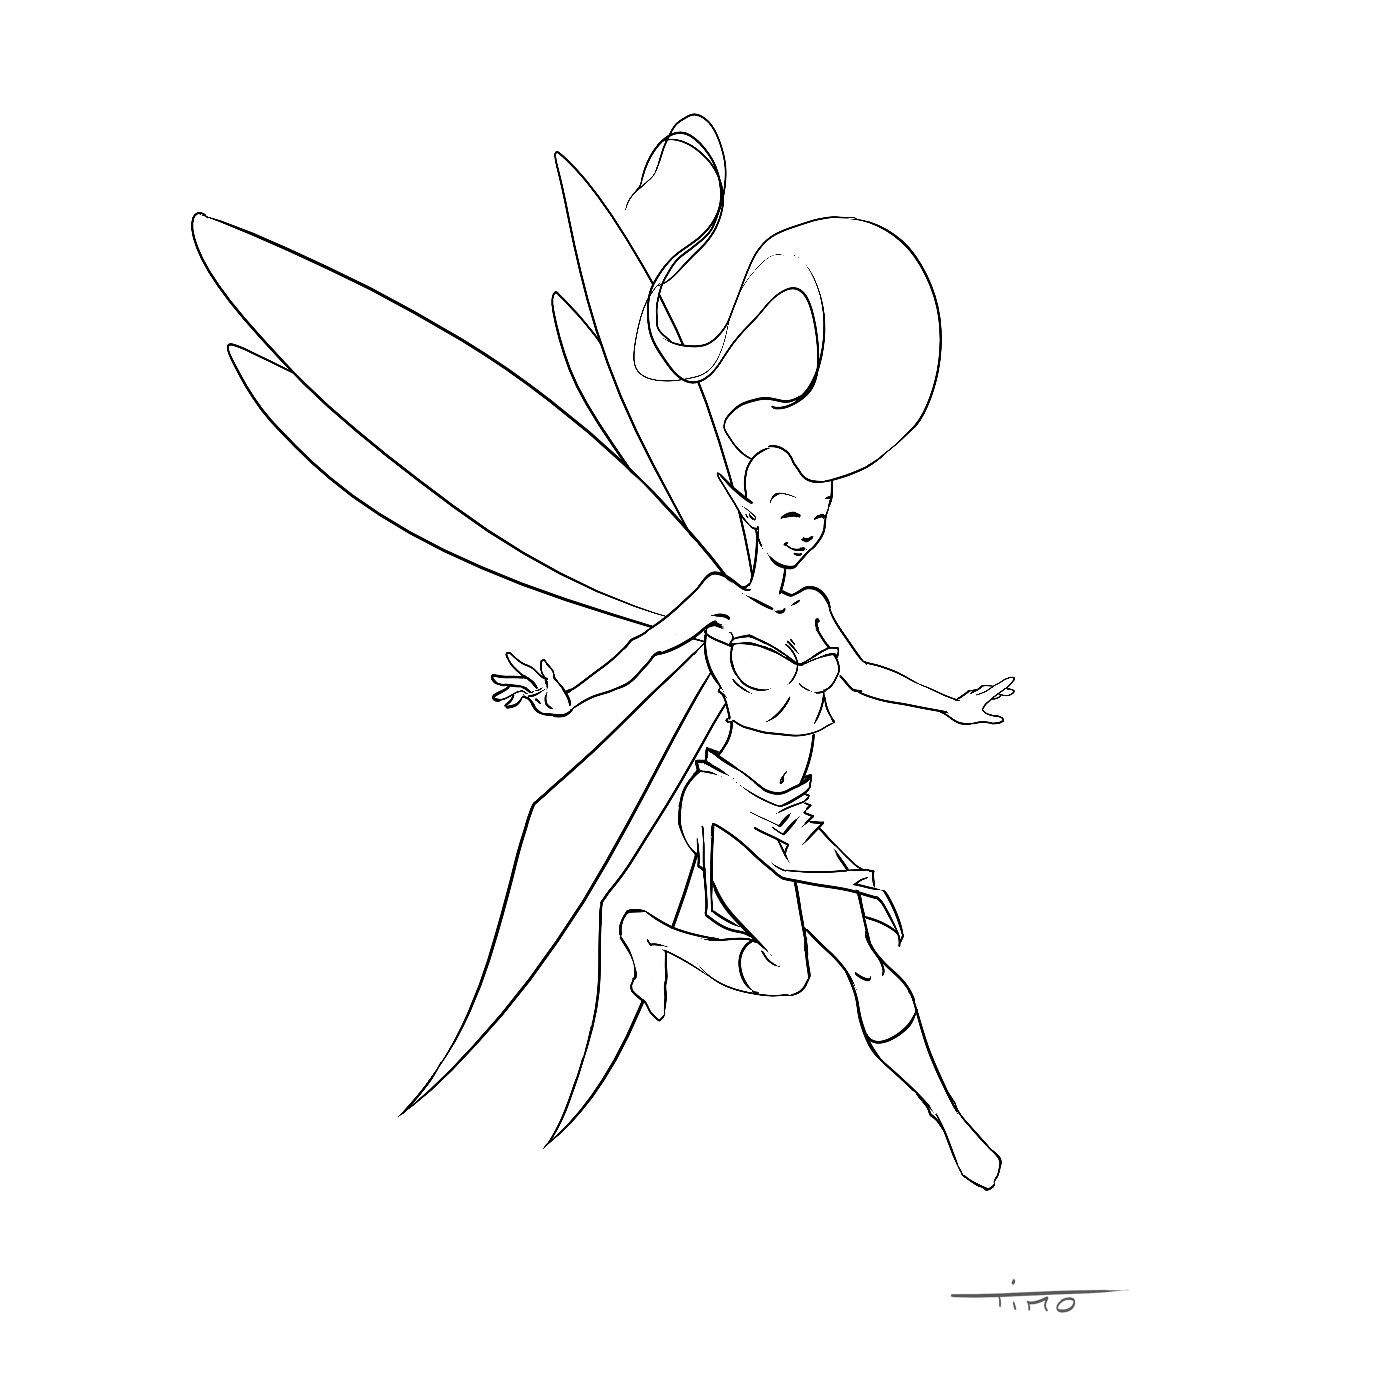
\includegraphics[scale=0.2,keepaspectratio=true]{./SeaFaery.png}
\end{center}
